\documentclass{exam}

\usepackage{graphicx}
\graphicspath{ {./images/} }

\lhead{ECON 2010}
\chead{Practice}
\lfoot{10/12/2023}
\rhead{Fall 2023}

% \printanswers
\noprintanswers

\begin{document}

\section{Practice Questions}

\begin{questions}

\question (E2 2021 Q4) John Maynard Keynes, a famous economist many of you will encounter in Econ 202, once wrote: ``In the long-run, we are all dead."  Putting aside Keynes' morbidity, let's think about the long run.

\begin{parts}
    \part In the space below, draw a long-run average cost curve (LRAC) that reflects “economies of scale,” “diseconomies of scale,” and “constant returns to scale.”  Label the portions that reflect the three different scale conditions.
    \vspace{2in}
    \part What would cause the entire LRAC curve to ``shift down''?
    \begin{solution}
        Lowering the cost of production, either from lower inputs costs or increasing productivity/technology.
    \end{solution}
\end{parts}

\question (E2 2020 Q2) The diagram below shows the cost curves of a competitive (i.e., perfectly competitive) firm.  This firm produces a product that currently has a market price of \$20.00.  Using economic logic, respond to the following questions.

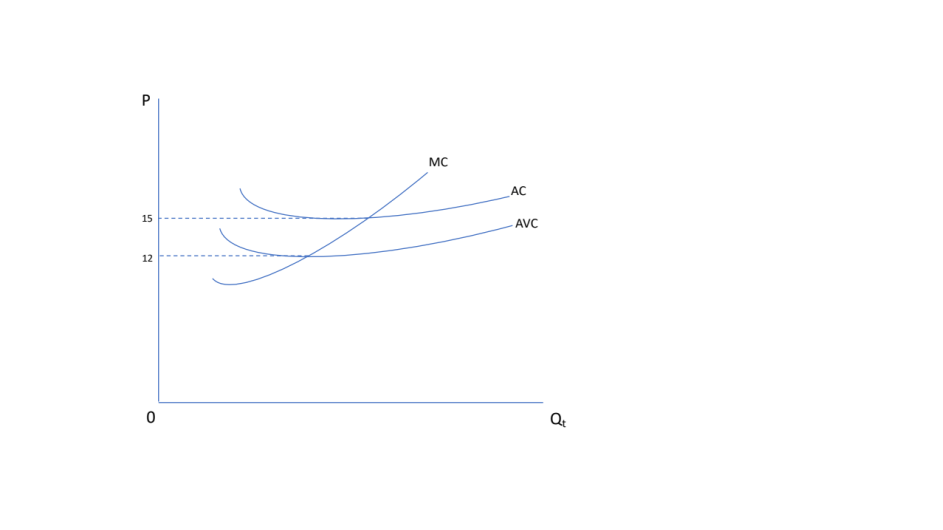
\includegraphics[width = \textwidth]{E2-2019Q4.png}

\begin{parts}
\part What will the demand curve facing this firm look like?
\begin{solution}
A perfectly competitive firm faces a horizontal demand curve. They may sell any amount of the good at the market price.
\end{solution}
\part What is the elasticity  of the demand curve this firm faces?
\begin{solution} 
The demand curve will be infinitely elastic. 
\end{solution}
\part Is the firm making economic profits or losses in the short run? Explain.
\begin{solution}
The firm is making economic profits. The firm will operate at the point where marginal revenue (\$20) is equal to marginal cost. Therefore, the firm is producing where marginal revenue exceeds average cost, indicating that they are profitable.
\end{solution}
\part How low would the market price have to fall before you would expect the owner of the firm to shut down and produce zero output?
\begin{solution} \$12 \end{solution}
\part Most of the firms in  this market have a similar cost structure to the one above. A trade journal for the industry claims that the current market price is not likely to continue in the long run (``expect a price collapse'' is the language that appeared in the trade journal). Do you agree with this prediction? Why or why not?
\begin{solution}
I agree. Firms in this industry are making economic profits. This will attract new entrants and increase the market supply curve, driving down the price. \end{solution}

\end{parts}

\question (E2 2020 Q5) Contrast the following economics terms with their definitions and/or a brief explanation:
\begin{parts}
\part Fixed versus variable cost.
\begin{solution}
Fixed costs are constant regardless of how much the firm produces. Variable costs depend on the level of production. Consider an Uber driver. The car is a fixed cost, while gasoline is a variable cost.
\end{solution}

\part Constant cost industry versus a decreasing cost industry

\begin{solution}
In the former, costs remain constant as production increases. In the latter, costs decrease as production increases.
\end{solution}

\part Gary Becker versus Daniel Kahneman.
\begin{solution}
Gary Becker describes consumers as inherently rational. He used consumer theory to describe many different aspects of human behavior. Daniel Kahneman believes that consumers can make mistakes due to behavioral biases.
\end{solution}

\part Pareto-optimal policy versus progressive taxation
\begin{solution}
A Pareto-optimal policy benefits some people and hurts no one. A progressive tax imposes a higher tax rate on individuals with higher incomes.
\end{solution}

\part Monopoly versus oligopoly.
\begin{solution}
In a monopoly, a single firm controls production of the good. In an oligopoly, a small number of firms control production.
\end{solution}

\part Supply curve for a competitive firm versus supply curve for a monopolist.
\begin{solution}
A competitive firm and a monopolist have the same supply curve: the portion of the marginal cost curve about the average variable cost curve.
\end{solution}

\part Dutch auction versus English auction.
\begin{solution} 
In a Dutch auction, the auctioneer starts at a high price and gradually lowers it until a bidder raises their hand. In an English auction, the auctioneer starts at a low price and raises it until only one bidder remains.
\end{solution}

\end{parts}

\end{questions}

\end{document}